\documentclass[11pt,answers]{exam}


\usepackage{graphicx}
\usepackage{amsmath}
\usepackage{color}
\usepackage{amssymb}
% \usepackage{setspace}
% \usepackage{epstopdf}
% \usepackage{empheq}
\usepackage{csquotes} % \textcquote
\usepackage{parskip}
% \setlength{\marginparwidth}{2cm}
% \usepackage{easyReview} % \alert, \highlight, \remove, \add, \replace, \comment
% \usepackage{subcaption}
% \usepackage[letterpaper]{geometry}
% \usepackage[definethebibliography]{easybib}
\usepackage{float}
\renewcommand{\solutiontitle}{\noindent\textbf{Authors Reply:}\par\noindent}

\usepackage{tikz}
\tikzstyle{block} = [rectangle, minimum width=2cm, minimum height=1cm,text centered, draw=black]
\tikzstyle{block_1} = [rectangle, minimum width=2cm, minimum height=1cm,text centered, draw=black, fill=blue!5]
\tikzstyle{block_2} = [rectangle, minimum width=2cm, minimum height=1cm,text centered, draw=black, fill=red!5]
\tikzstyle{arrow} = [thick,->,>=stealth]
\tikzstyle{arrow_2} = [very thick,->,>=stealth]
\tikzstyle{arrow_3} = [thick,->,>=stealth,dashed]
\tikzstyle{pfr} = [cylinder, draw, minimum height=4cm, minimum width=1cm, shape aspect=1, shape border rotate=180]
\usetikzlibrary{shapes.geometric}

% \renewcommand{\sectionmark}[1]{\rightmark{#1}}

% \header{}{}{title: \rightmark}
\footer{}{Page \thepage\ of \numpages}{}

\begin{document}

\section*{first page}
 
First page intentionally left blank.
 
\newpage

\section*{Reviewer 1}
% \thispagestyle{headandfoot}

The comments of Reviewer 1, along with our responses to each comment, are included below:

\begin{quote}
    \textquote{This work presents a boundary optimal control strategy for axial tubular reactors with first-order irreversible chemical reaction incorporating a delayed recycle stream. The mathematical description takes the form of a system of coupled parabolic and hyperbolic PDEs. An infinite-dimensional approach is applied to derive a linear quadratic regulator with and without observer. Numerical studies show that the proposed controller is able to stabilize the system. The manuscript is clear and well written and addresses a challenging control problem in chemical engineering. The following comments and suggestions may improve the presentation so that it is considered for publication.}
\end{quote}

\begin{questions}

    \question Page 3 - \textquote{Many chemical, petrochemical, and biochemical unit operation processes are modelled as
    distributed parameter systems (DPS).}

    A few specific examples of these chemical processes would help to motivate the problem this paper addresses

    \begin{solutionorbox} \label{comment:1_1}
        Examples have been added to the introduction and the manuscript has been revised accordingly.
    \end{solutionorbox}

    \question Page 5 - \textquote{PIDEs}

    - What does PIDEs stand for?

    \begin{solutionorbox} \label{comment:1_2}
        We thank the reviewer for this suggestion. It stands for Partial Integro Differential Equations. The acronym has now been defined in the manuscript and the manuscript has been revised accordingly.
    \end{solutionorbox}


    \question Page 5 - \textquote{a configuration common in industrial processes}

    - Examples of these processes would illustrate the need and motivation to address the associated
    control problem

    \begin{solutionorbox} \label{comment:1_3}
        Examples have been added to the introduction and the manuscript has been revised accordingly.
    \end{solutionorbox}


    \question Page 6 - \textquote{The resulting PDE that describes the reactor model is given by:}

    - I suggest to specify the assumptions leading to the reactor model, like isothermal operation,
    constant properties, constant pressure, ...

    \begin{solutionorbox} \label{comment:1_4}
        We appreciate the reviewer’s suggestion to clarify the assumptions underlying the reactor model. Based on feedback from multiple reviewers, we recognize that the modeling section in the original manuscript was brief and may have caused misunderstandings, as it focused primarily on building a general framework rather than providing detailed explanations.

        To address these issues, we have revised the modeling section to provide a more detailed and comprehensive explanation while maintaining the generality of the proposed framework. As part of these updates, it is now explicitly mentioned in the revised manuscript that the model assumes the parameters of the system are constant and thus, the states of the system are not affected by changes in system's pressure or temperature.
    \end{solutionorbox}


    \question Page 7 - Eq (2)

    - What is the physical meaning of the manipulated variable $u(t)$?

    \begin{solutionorbox} \label{comment:1_5}
        As the result of the changes made in the modelling section of the manuscript, the manipulated variable $u(t)$ is of the same nature as the system's states, i.e. deviation of the reactant concentrations from its steady-state in the reactor feed stream. The manuscript has been updated to address this point. These changes are further discussed in Comment~\ref{comment:1_11}.
    \end{solutionorbox}


    \question Page 7 - \textquote{ $x_2(\zeta, t)$ is introduced as a new state variable to account for the concentration along the recycle stream}

    - Why is $x_2$ a function of $\zeta$ ? How does $x_2$ change across the recycle? What kind of law does it follow? To me, it seems like $x_2$ only changes with respect to time

    \begin{solutionorbox} \label{comment:1_6}
        We have assumed that along the recycle stream, the flow of the reactant belongs to the class of pure transport PDEs. This is the case when the diffusion term and the reaction term become negligible compared to the convective term, and the state variable $x_2$ is merely being transported along the recycle stream. Nevertheless, this still implies that $x_2$ is a function of $\zeta$ and $t$. Concentration profile along the recycle stream has not been presented in the original submission as we believe it is not the focus of this work. However, for the reviewer's reference, it is included here in the response as shown in Fig.~\ref{fig:x2}.
    \end{solutionorbox}

\begin{figure}[H]
    \centering
    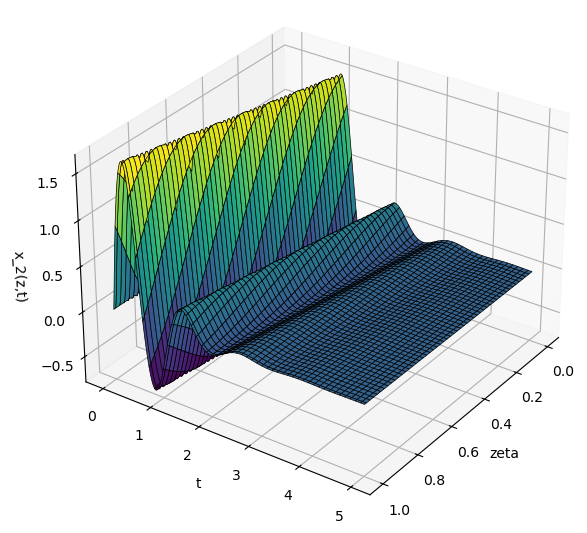
\includegraphics[width=0.65\textwidth]{x2_vs_z.png}
    \caption{Concentration profile along the recycle stream}
    \label{fig:x2}
\end{figure}

    \question Page 8 - Eq (5)
    
    - Please make a distinction between the symbol for domain and for diffusivity to avoid confusion

    \begin{solutionorbox} \label{comment:1_7'}
        We appreciate the reviewer's suggestion. We have replaced the symbol for the domain with $\mathcal{D}$ to avoid confusion. The manuscript has been updated accordingly.
    \end{solutionorbox}


    \question Page 12 - Riesz-spectral operator $\mathfrak{A}$

    - Although a rigorous proof is not necessary, it would be good if the authors explain why $\mathfrak{A}$ is a Riesz-spectral operator. I guess its eigenvalues and eigenfunctions satisfy the requirements, like having multiplicity one and forming a Riesz basis, respectively.

    \begin{solutionorbox} \label{comment:1_8}
        That, along with the fact that the obtained set of eigenfunctions for $\mathfrak{A}$ and $\mathfrak{A}^*$ seem to form a bi-orthogonal basis that can successfully span the state space, is the reason behind this statement. By obtaining the spectrum for the system generator and its adjoint, followed by properly scaling the eigenfunctions, we observe that the aforementioned properties are satisfied. To be more specific, the inner products of $\phi_i$ and $\psi_j$ gives $\delta_{i,j}$, and every arbitrary function that satisfies the domain may be expressed as a linear combination of the given bi-orthogonal basis.
    \end{solutionorbox}


    \question Page 12 - $\mathfrak{R}$ being positive semi-definite operator

    - Should $\mathfrak{R}$ be self-adjoint and coercive?

    \begin{solutionorbox} \label{comment:1_9}
        The authors appreciate the reviewer for mentioning this. According to \cite{curtainbook} for the infinite-dimensional LQR problem on the infinite-time interval, operator $\mathfrak{R}$ should be self-adjoint and coercive, which is a better way to address the operator compared to self-adjoint and positive semi-definite. Since the system has finite-dimensional (to be more specific, scalar in this case) real input, these two sets of conditions will be identical; yet to enhance the quality of the work, reviewer's suggestion has been taken into consideration and the manuscript has been updated accordingly.
    \end{solutionorbox}


    \question Page 12 - The LQR problem

    - Is Problem 12 well-posed, does J have a finite value for at least one u?

    \begin{solutionorbox} \label{comment:1_10}
        The proposed infinite-time LQR problem is well-posed, i.e. for at least one input trajectory $u(t)$, the infinite-time cost function $J$ has a finite value. The stabilizing input trajectory obtained in the manuscript is an example as all the eigenvalues of the obtained closed-loop system $\mathfrak{A} - \mathfrak{B} K$ are in the open left half of the complex plane. 
    \end{solutionorbox}


    \question Page 18 - unstable dynamics of the model

    - Why is the zero-input response considered unstable? Is it a qualitatively assessment? What is the physical meaning of Figure 9?

    \begin{solutionorbox} \label{comment:1_11}
        We appreciate the reviewer’s thoughtful questions regarding the zero-input response and its interpretation. As mentioned previously, the original submission focused on the broader goals of the study, offering a concise explanation of the proposed model. However, based on the reviewers’ feedback, we recognized the need to address potential misunderstandings caused by this brevity. To address this query comprehensively, we aim to clarify the modeling approach by outlining the modeling steps and the reasoning behind the chosen framework here in the reply, as they are critical for understanding the observed instability and its implications. In addition, we have also updated the manuscript to provide a more detailed and general explanation of the model. These revisions ensure that the manuscript presents a clearer and more comprehensive framework while preserving the original model’s intent and structure.
        
        For the axial dispersion tubular reactor presented in Fig.~\ref{fig:reactor}, the molar balance equation may be written for the reactant concentration, $C_A$, as follows:
        
        \begin{equation}
            \frac{\partial C_A}{\partial t} = D \frac{\partial^2 C_A}{\partial \zeta^2} - v \frac{\partial C_A}{\partial \zeta} - r(C_A)
        \end{equation}
        
        where $r(C_A)$ is the reaction rate by which the reactant is consumed. Considering this term can be non-linear, the model can be linearized around the steady-state followed by replacing the state of the system with deviation from the steady-state concentration. This will result in the following equation:
        
        \begin{equation}
            \frac{\partial \epsilon}{\partial t} = D \frac{\partial^2 \epsilon}{\partial \zeta^2} - v \frac{\partial \epsilon}{\partial \zeta} - \left( \left. \frac{\partial r(C_A)}{\partial C_A} \right|_{C_{A, ss}} \right) \epsilon
        \end{equation}
        
        Here, $\epsilon \equiv C_A - C_{A, ss}$ is the deviation from the steady-state concentration, and $C_{A, ss}$ is the steady-state concentration of the reactant. The stability analysis of the system in the vicinity of the steady state has been one of the first things of our interest. 
        
        While no isothermal reactor can technically be exponentially unstable due to the finite amount of reactant available, such systems can be unstable in the vicinity of the steady state, meaning that a deviation from the steady state may draw the states of the system to a different steady state, resulting in completely different model dynamics than the one used to design and control the system for optimal operation.
        
        Performing the eigenvalue analysis of the system, we have observed that a system may have unstable steady-state only when the reaction term coefficient $-\frac{\partial r(C_A)}{\partial C_A}$ is positive around a given steady-state. Though an uncommon scenario, this may happen in the case of autocatalytic reactions, enzyme-catalyzed reactions, reactions that incorporate inhibition mechanisms, etc. Although the proposed controller can also stabilize an already stable system in an optimal manner, a positive reaction term is intentionally selected to demonstrate the ability of the proposed controller to stabilize a system which is mathematically unstable. We believe that such aspect of the controller has to be inspected within the general framework of the controller proposed in this work as it becomes more significant when the work is extended to more complex systems where instability becomes a common issue.

        As a result, the zero-input response is considered unstable due to the positive reaction term in the model. Figure 9 illustrates the unstable dynamics of the linearized model in the vicinity of the steady-state in the absence of control input; with the qualitative assessment that a deviation from the steady state may draw the system to a different steady state, resulting in completely different model dynamics than the one used to design and control the system for optimal operation. The manuscript has been updated to include more detailed explanation in this regard.
    \end{solutionorbox}

    \begin{figure}[H]
        \centering
        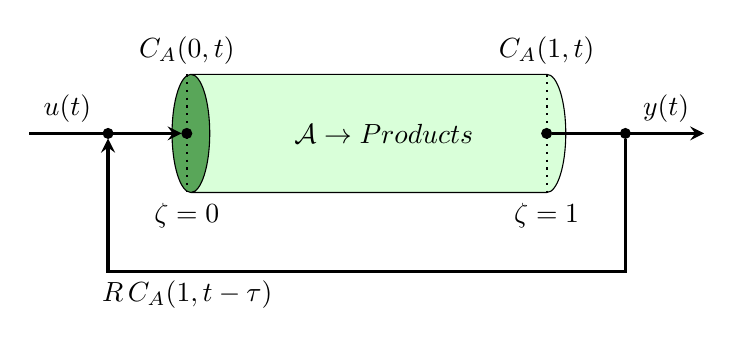
\begin{tikzpicture}
            \node (pfr) [cylinder, draw, minimum height=5cm, minimum width=1.5cm, shape aspect=1, shape border rotate=180, cylinder uses custom fill, cylinder end fill=green!30!gray, cylinder body fill=green!15] {$\mathcal{A} \rightarrow {Products}$};
            \node (pfr_inlet) [circle, left of=pfr, xshift=-1.5cm, fill=black, draw, inner sep=0pt, minimum size=0.25cm, scale=0.5] {};
            \node (pfr_outlet) [circle, at={(pfr.east)}, shift={(-0.25cm,0)}, fill=black, draw, inner sep=0pt, minimum size=0.25cm, scale=0.5] {};
            \node (recycle_right) [circle, right of=pfr_outlet, fill=black, draw, inner sep=0pt, minimum size=0.25cm, scale=0.5] {};
            \node (recycle_left) [circle, left of=pfr_inlet, fill=black, draw, inner sep=0pt, minimum size=0.25cm, scale=0.5] {};
        
            \draw[dotted, thick] ([yshift=0.75cm]pfr_inlet.center) -- node[at end, below, yshift=0cm] {$\zeta = 0$} ([yshift=-0.75cm]pfr_inlet.center);
            \draw[dotted, thick] ([yshift=0.75cm]pfr_outlet.center) -- node[at end, below, yshift=0cm] {$\zeta = 1$} ([yshift=-0.75cm]pfr_outlet.center);
        
            \node[below of=recycle_left, node distance=1.75cm, anchor=north west, xshift=-0.2cm] {$R \, C_A(1, t-\tau)$};
            \node[above of=pfr_inlet, node distance=1.05cm,] {$C_A(0, t)$};
            \node[above of=pfr_outlet, node distance=1.05cm,] {$C_A(1, t)$};
            
            \draw [arrow_2] (pfr_outlet) -- node[near end, above] {$y(t)$} ++(2,0);
            \draw [arrow_2] (pfr_inlet) ++(-2,0) coordinate(start) -- node[near start, above] {$u(t)$} (pfr_inlet);
            \draw [arrow_2] (recycle_right) -- ++(0,-1.75) -| (recycle_left);
            
        \end{tikzpicture}
        \caption{Axial tubular reactor with recycle stream.}
        \label{fig:reactor}
    \end{figure}

    \question Page 18 - \textquote{The goal is to stabilize the system using an optimal control strategy}

    - What are the values of matrices Q and R in the objective function?

    \begin{solutionorbox} \label{comment:1_12}
        The authors thank the reviewer for their comment on this matter. The values for operators $\mathfrak{Q}$ and $\mathfrak{R}$ in the objective function were not explicitly mentioned in the manuscript. These values are chosen as $\mathfrak{Q} = 0.05 \times \mathfrak{I}$ and $\mathfrak{R} = 50$, where $\mathfrak{I}$ is the identity operator of the same size as $\mathfrak{A}$. The manuscript has been updated accordingly.
    \end{solutionorbox}


    \question Page 18 - \textquote{The goal is to stabilize the system using an optimal control strategy}

    - Are x deviation variables? What is the setpoint?

    \begin{solutionorbox} \label{comment:1_13}
        The state variable $x(\zeta,t)$ is the deviation of the reactant concentration from its steady-state in the reactor. The setpoint is therefore zero, as the goal is to stabilize the system around the steady-state. The manuscript has been updated accordingly.
    \end{solutionorbox}


    \question Page 20 - \textquote{Both optimal feedback gains are able to successfully stabilize the system within finite time horizon.}

    - It would be interesting to see how the delay time affects the stabilizing capabilities of the feedback regulator. What would happen a shorter and larger values of $\tau$

    \begin{solutionorbox} \label{comment:1_14}
        We thank the reviewer for their suggestion to explore how variations in the delay time (\(\tau\)) affect the stabilizing capabilities of the feedback regulator. During the course of this work, we observed that parameter sensitivity analysis naturally raises reader curiosity, as reflected in the diverse interests of all reviewers. For instance, some reviewers were interested in parameters like the Peclet number or recycle ratio, while others focused on \(\tau\). This breadth highlights how sensitivity analysis could easily expand beyond the intended scope of this study.

        While we were initially hesitant to include detailed sensitivity analysis to maintain the focus of the work, we decided to investigate \(\tau\) specifically, as it is directly tied to the delay-based dynamics central to this study. This decision was made to further strengthen the work and to address the natural curiosity of readers about this critical parameter. A new figure has been added to the revised manuscript, illustrating how the controller’s performance varies with changes in \(\tau\), and the discussion has been updated to reflect these findings. 
    \end{solutionorbox}


    \question Page 26 - \textquote{The proposed framework may be extended to more complex diffusion convection reactor configurations, such as non-isothermal reactors}

    - Can this framework be applied to reaction systems described with more complex and highly nonlinear reaction kinetics?

    \begin{solutionorbox} \label{comment:1_15}
        The authors thank the reviewer for their comment. According to the changes made in the model mentioned in Comment~\ref{comment:1_11}, a general non-linear reaction kinetics is now considered in the model. The manuscript has been updated accordingly.

        It is worth mentioning that even after considering a general non-linear reaction kinetics, the proposed framework is applied to the linearized representation of the system model around its steady state, as non-linear models are not guaranteed to have solutions.
    \end{solutionorbox}


\end{questions}

\newpage

\section*{Reviewer 2}

The comments of Reviewer 2, along with our responses to each comment, are included below:

\begin{quote}
    ``The problem presented in the article is well-posed and written. The purpose is to present a novel approach to address the problem of intrinsic delay when there is a recycle stream in a process. However, I recommend submitting it to a journal focused on Control. This opinion is based on the following concerns regarding the process of a chemical reactor with recycle:''
\end{quote}


\begin{questions}

    \question Why is relevant to consider Danckwerts boundary conditions for the problem of control? Have you compared your results with those obtained considering other boundary conditions?

    \begin{solutionorbox} \label{comment:2_1}
        The authors appreciate the reviewer's concern regarding the choice of boundary conditions. In the field of chemical engineering process control and dynamics, the Danckwerts boundary condition has become an inseparable part of the modeling procedure when it comes to tubular reactors. Belonging to the class of Robin boundary conditions, the choice of Danckwerts boundary condition maintains generality while capturing physical significance without simplifying the problem. Therefore, although considering other boundary conditions is a possibility, they may lack the physical relevance and generality offered by the Danckwerts condition in this context. The manuscript has been updated to include a brief explanation of the choice of boundary conditions.
    \end{solutionorbox}


    \question Concerning the recycle stream, have you studied the effect of the R, the recycle ratio, on your results? Please comment.

    \begin{solutionorbox} \label{comment:2_2}
        The effect of the recycle ratio has been studied on the dynamics of the system and the performance of the controller during the initial simulations. We observed that as \( R \to 1 \), the open-loop system behaves more like a CSTR (i.e., concentration profiles start to become flat). However, it becomes more challenging for the controller to stabilize the system, likely because the controller action is significantly diluted at the reactor inlet after being mixed with the recycle stream.

        Parameter sensitivity analysis naturally raises reader curiosity, as reflected in the diverse interests of all reviewers. For example, some reviewers focused on the Peclet number or delay time (\( \tau \)), while others, like the reviewer here, were interested in the recycle ratio (\( R \)). This diversity highlights how sensitivity analysis could quickly expand beyond the intended scope of this work. While we were initially hesitant to include detailed sensitivity analysis to maintain the focus of the work, and although we acknowledge the importance of \( R \) in influencing system behavior, we decided to pick \( \tau \) among all parameters because it is central to our work and directly tied to the delay-based dynamics being studied, and to address the natural curiosity of readers. Expanding the analysis to include other parameters, such as \( R \), would risk exceeding the intended scope. By narrowing our focus, we aimed to address the natural curiosity of readers while maintaining the study's clarity and precision. Nevertheless, a brief discussion on the effect of the recycle ratio on the system dynamics has been added to the revised manuscript, but a detailed sensitivity analysis on \( R \) has not been included.
        
        It is worth noting that, throughout this work, the proposed modeling and control strategy has been demonstrated to effectively stabilize a wide range of parameter sets, including variations in the recycle ratio. This ensures the adaptability of the proposed control strategy across diverse system configurations.
    \end{solutionorbox}

    
    \question The authors used as the case study the problem of an axial dispersion tubular reactor incorporating diffusion, convection, and a first-order irreversible chemical reaction described by equations (1)-(2). While this is sufficient to present their approach, it is far from being extended to the more general problem, non-isothermal, and with more general kinetics such as biochemical or catalytic.

    \begin{solutionorbox} \label{comment:2_3}
        The authors appreciate the insightful comment. In response, we have taken the following steps to clarify how our current framework, while based on simplified assumptions, is inherently flexible and can accommodate further complexities without requiring significant changes to its structure. 

        \begin{enumerate}
            \item \textbf{General Reaction Kinetics:} Regarding the general kinetics within the proposed model, we have revised the manuscript to demonstrate how a generalized reaction term \( r = r(C_A) \), where \( C_A \) is the reactant concentration, can be incorporated within the proposed framework. This change ensures that the model can accommodate a broad range of reaction kinetics while maintaining its core focus.
            
            \item \textbf{Non-Isothermal Case:} We agree that temperature dependence can significantly impact reactor dynamics. In fact, as a natural extension of this work, we are already working on addressing the non-isothermal case in a separate submission to the \textit{Canadian Journal of Chemical Engineering}. This future study builds on the foundation established here, demonstrating the potential flexibility of the proposed framework as the inclusion of thermal effects and their influence on system dynamics will fit seamlessly into the same model structure.
        \end{enumerate}

        We emphasize that the primary objective of this study is to establish a foundational framework addressing intrinsic delays in distributed parameter systems (DPS) for process control and dynamics. More detailed and physically specific extensions, such as those involving non-isothermal behavior or highly nonlinear kinetics, are intentionally reserved for subsequent studies to build upon this foundation.       
    \end{solutionorbox}


    \question I recommend submitting it to a journal focused on Control.

    \begin{solutionorbox} \label{comment:2_4}
        We appreciate the suggestion to submit this work to a control-focused journal. However, we believe this study is best suited for a chemical engineering journal because it contributes meaningfully to process control and dynamics within the unique context of chemical engineering rather than the general domain of control theory.

        Chemical engineering inherently incorporates process control and dynamics, making the two disciplines inseparable. While this work is centered around proposing a control strategy, its significance is rooted in the unique context of chemical engineering process control, where state delays are rarely addressed. Although state delays have been extensively studied in other fields with different system models, applying such a strategy to chemical engineering systems—particularly those convection-diffusion-reaction DPSs described by second order PDEs—is novel and valuable. 
        
        Furthermore, we would like to emphasize that similar research \cite{li2024novel, azhin2021modelling} has been recently published in the \textit{Canadian Journal of Chemical Engineering}, demonstrating contributions to control theory that align with those presented in our work. This validates the relevance of publishing control-focused studies within chemical engineering journals, which often encompass modeling and novel methodologies essential to the field.

        On top of that, we are planning to extend this work in our upcoming submissions to the \textit{Canadian Journal of Chemical Engineering} by addressing temperature dependence of the reaction rates, which will be built on the foundation laid by this study. This extension will further enhance the practical implications of our findings, emphasizing the broader impact of this study on chemical engineering practice. All of these aspects makes us confident that this work is well aligned with the scope and readership of this journal.
    \end{solutionorbox}

\end{questions}

% Reviewing: 3
\newpage
\section*{Reviewer 3}

The comments of Reviewer 3, along with our responses to each comment, are included below:

\begin{quote}
    ``In this work, the authors address the optimal control of an axial tubular reactor with a recycle stream. They model the intrinsic time delay from the recycling process using a system of coupled parabolic and hyperbolic partial differential equations. The control input is applied at the inlet, and a continuous-time optimal linear quadratic regulator is designed to stabilize the system. Numerical simulations indicate effective full-state feedback regulator and observer-based regulator. This work presents an interesting methodology but there are some minor considerations that the authors need to address before this article can be published:''
\end{quote}

\begin{questions}

    \question \textbf{Major comment: } In section 4, the authors indicate that they discretized each state in space using 100 grid points. They must indicate if those points are equidistributed and how they came up with such discretization grid. Note that multiple works \cite{palma2023selection, assassa2016optimality, chen2014bilevel} have demonstrated that the selection and distribution of the discretization grid plays a crucial role in the computation of optimal control laws, i.e., a control law can be claimed to be optimal or not using the criterion of the Pontryagin's Minimum Principle (PMP). The reviewer recommends to assess the criterion of the Hamiltonian function (i.e., the PMP) to demonstrate that the discretization implemented is accurate and the solutions obtained for the control are optimal.

    \begin{solutionorbox} \label{comment:3_1}
        The authors thank the reviewer for the insightful and detailed comment. We have gone through the suggested literature and agree that the selection and distribution of the discretization grid are crucial in converting an infinite-dimensional system to a finite-dimensional one. However, we would also like to point out that based on the late-lumping approach used in the proposed work, we do not discretize the system in space at all. In fact, the infinite-dimensional nature of the system is fully captured in the proposed control strategy, and the control law is designed directly in the infinite-dimensional space.

        The 100 grid points mentioned in the manuscript are merely used to confirm how the optimal control input will be applied to the system. In other words, the feedback gain is designed based on the infinite-dimensional system, and the control input is obtained with no need for spatial discretization. It is only at this point that the obtained control input is applied to a FDM representation of the system to evaluate the system's response to the control input. Nevertheless, the 100 grid points are equidistributed, and the discretization grid is uniform. The manuscript has been updated accordingly to both clarify this point and explain the rationale behind the grid points.
    \end{solutionorbox}


    \question The manuscript lacks conclusions or further discussion about the control trajectories' results, such as the quality of the control actions or improvements in process operation (e.g., avoidance of constraint violations, disturbance rejection, etc.). Although the authors included several figures illustrating the process dynamics and control trajectories, these are not discussed in sufficient depth, i.e., avoid leaving the reader to draw their own conclusions from the figures. Additionally, the reviewer recommends reducing the number of figures, which could allow more space for further discussion of the results.

    \begin{solutionorbox} \label{comment:3_2}
        The reviewer's suggestion is well taken, and further discussion of the results has been added to the revised manuscript. With the inclusion of parameter sensitivity analysis as discussed in Comment~\ref{comment:3_3}, there is now more room to discuss the controller's performance in more detail. In addition, Figure 9 (open-loop unstable system state response) has been removed accordingly, as the stability analysis has been discussed separately in detail in the revised manuscript. 

        Nevertheless, regarding the requested improvements offered by the proposed controller (e.g., disturbance rejection or constrained input/output), we emphasize that this work is rather foundational, focusing on stabilization as a prerequisite for higher-level control objectives such as the servo or regulatory problem. Stabilization ensures predictable system behavior, which is essential for implementing advanced control strategies.
        
        We are currently extending this work to address temperature dependence of the reaction rates, with plans for submission to the \textit{Canadian Journal of Chemical Engineering}. Building on the modeling and control strategy introduced here, we also aim to address the regulatory problem (i.e., rejecting disturbances and maintaining the system at a desired setpoint). Furthermore, to incorporate constrained input/output, we can transition to discrete-time MPC in future work, showcasing how the foundations laid in this study can be expanded to address more complex modeling and control challenges.
    \end{solutionorbox}


    \question In section 3.1.3, the authors present the values for parameters R and D but provide no further details about the model's sensitivity to these parameters. Please include a detailed explanation of how these values were selected and discuss any potential limitations if the parameters are chosen incorrectly.

    \begin{solutionorbox} \label{comment:3_3}
        The effects of the recycle ratio (\(R\)) and the diffusivity coefficient (\(D\)) on the system dynamics and controller performance were explored during initial simulations. For instance, as \(R \to 1\), the open-loop system exhibits behavior akin to a CSTR, with concentration profiles flattening. However, this increases the challenge of stabilizing the system, as the controller's action becomes diluted at the reactor inlet due to mixing with the recycle stream. Similarly, an increase in the diffusivity coefficient (or a decrease in the Peclet number) causes the eigenvalues of the system generator to shift closer to the real axis. This implies that greater diffusion within the reactor dampens oscillatory dynamics introduced by the delayed recycle stream.

        While parameter sensitivity analysis is important and naturally raises curiosity, as seen from the diverse interests of the reviewers (e.g., Peclet number, delay time, recycle ratio), expanding the analysis to include all parameters would risk exceeding the intended scope of this work. To address reader's curiosity, we decided to focus on \( \tau \) among all parameters as it is central to the delay-based dynamics being studied and directly tied to the novel modeling and control strategy we propose. While the Peclet number and recycle ratio certainly influence system behavior, they do not directly affect the core contributions of this work, which is to offer a novel modeling and control framework for a certain class of distributed parameter systems in chemical engineering. Nevertheless, a brief discussion on the effect of the diffusion coefficient $D$ on the system dynamics has been added to the revised manuscript, but a detailed sensitivity analysis on \( D \) has not been included.
    
        It is worth emphasizing that the proposed modeling and control strategy has been shown to effectively stabilize the system over a broad range of parameter sets, including variations in the Peclet number and recycle ratio. This adaptability ensures the practicality of the proposed framework across different system configurations.
    \end{solutionorbox}


    \question In section 4, the authors indicate that the process model was discretized in time and space, however, they mention that they obtained a system of ordinary differential equations (ODEs). Please clarify how this full discretization resulted in a system of ODEs.

    \begin{solutionorbox} \label{comment:3_4}
        The authors appreciate the reviewer for pointing out this issue. We acknowledge that the manuscript appears to be ambiguous in this regard. The authors clarify that the ODEs are obtained as a result of applying space discretization to the infinite-dimensional system (as previously explained in comment~\ref{comment:3_1}). To solve the system of ODEs with respect to time, we used the numerical solver mentioned in the manuscript, indicating that the numerical solver inherently applies time discretization. The manuscript has been updated to address this point.
    \end{solutionorbox}

    \question The manuscript has some typos that the authors must correct, e.g., …setting for of distributed…, Then two full-state… In page 5, the acronym PIDEs is not previously defined. For section 4.3, the reviewer recommends to modify the expression “Last but not least” aiming not loose the formality of the manuscript.

    \begin{solutionorbox} \label{comment:3_5}
        We appreciate the reviewer’s detailed observations and have addressed their suggestions.
    \end{solutionorbox}


    \question The reviewer recommends to include a tables of nomenclature

    \begin{solutionorbox} \label{comment:3_6}
        A complete table of nomenclature has been included in the revised manuscript.
    \end{solutionorbox}
\end{questions}


\newpage
\bibliographystyle{vancouver}
\bibliography{references.bib}
\end{document}